%%%%%%%%%%%%%%%%%%%%%%%%%%%%%%%%%%%%%%%%%
% Beamer Presentation
% LaTeX Template
% Version 1.0 (10/11/12)
%
% This template has been downloaded from:
% http://www.LaTeXTemplates.com
%
% License:
% CC BY-NC-SA 3.0 (http://creativecommons.org/licenses/by-nc-sa/3.0/)
%
%%%%%%%%%%%%%%%%%%%%%%%%%%%%%%%%%%%%%%%%%

%----------------------------------------------------------------------------------------
%	PACKAGES AND THEMES
%----------------------------------------------------------------------------------------

\documentclass{beamer}
\AtBeginSection[]
{
  \begin{frame}
    \frametitle{Table of Contents}
    \tableofcontents[currentsection]
  \end{frame}
}
\newenvironment<>{varblock}[2][.9\textwidth]{%
  \setlength{\textwidth}{#1}
  \begin{actionenv}#3%
    \def\insertblocktitle{#2}%
    \par%
    \usebeamertemplate{block begin}}
  {\par%
    \usebeamertemplate{block end}%
  \end{actionenv}}
  
\mode<presentation> {

% The Beamer class comes with a number of default slide themes
% which change the colors and layouts of slides. Below this is a list
% of all the themes, uncomment each in turn to see what they look like.

%\usetheme{default}
%\usetheme{AnnArbor}
%\usetheme{Antibes}
%\usetheme{Bergen}
%\usetheme{Berkeley}
%\usetheme{Berlin}
%\usetheme{Boadilla}
%\usetheme{CambridgeUS}
%\usetheme{Copenhagen}
%\usetheme{Darmstadt}
%\usetheme{Dresden}
%\usetheme{Frankfurt}
%\usetheme{Goettingen}
%\usetheme{Hannover}
%\usetheme{Ilmenau}
%\usetheme{JuanLesPins}
%\usetheme{Luebeck}
\usetheme{Madrid}
%\usetheme{Malmoe}
%\usetheme{Marburg}
%\usetheme{Montpellier}
%\usetheme{PaloAlto}
%\usetheme{Pittsburgh}
%\usetheme{Rochester}
%\usetheme{Singapore}
%\usetheme{Szeged}
%\usetheme{Warsaw}

% As well as themes, the Beamer class has a number of color themes
% for any slide theme. Uncomment each of these in turn to see how it
% changes the colors of your current slide theme.

%\usecolortheme{albatross}
%\usecolortheme{beaver}
%\usecolortheme{beetle}
%\usecolortheme{crane}
%\usecolortheme{dolphin}
%\usecolortheme{dove}
%\usecolortheme{fly}
%\usecolortheme{lily}
%\usecolortheme{orchid}
%\usecolortheme{rose}
%\usecolortheme{seagull}
%\usecolortheme{seahorse}
%\usecolortheme{whale}
%\usecolortheme{wolverine}

%\setbeamertemplate{footline} % To remove the footer line in all slides uncomment this line
%\setbeamertemplate{footline}[page number] % To replace the footer line in all slides with a simple slide count uncomment this line

%\setbeamertemplate{navigation symbols}{} % To remove the navigation symbols from the bottom of all slides uncomment this line
}

\usepackage{graphicx} % Allows including images
\usepackage{booktabs} % Allows the use of \toprule, \midrule and \bottomrule in tables
\usepackage{verbatim}
\usepackage{minted}
\usepackage{xcolor}
\usepackage{color}

\usepackage{listings}% http://ctan.org/pkg/listings
\usepackage{xcolor}% http://ctan.org/pkg/xcolor
\definecolor{bluekeywords}{rgb}{0.13,0.13,1}
\definecolor{greencomments}{rgb}{0,0.5,0}
\definecolor{turqusnumbers}{rgb}{0.17,0.57,0.69}
\definecolor{redstrings}{rgb}{0.5,0,0}


\lstdefinelanguage{FSharp}
    {morekeywords={let, new, match, with, rec, open, module, namespace, type, of, member, and, for, in, do, begin, end, fun, function, try, mutable, if, then, else},
    keywordstyle=\color{bluekeywords},
    sensitive=false,
    morecomment=[l][\color{greencomments}]{///},
    morecomment=[l][\color{greencomments}]{//},
    morecomment=[s][\color{greencomments}]{{(*}{*)}},
    morestring=[b]",
    stringstyle=\color{redstrings}
    }

\lstnewenvironment{fslisting}
  {
    \lstset{
        language=FSharp,
        basicstyle=\ttfamily,
        breaklines=true,
        columns=fullflexible}
  }
  {
  }

%----------------------------------------------------------------------------------------
%	TITLE PAGE
%----------------------------------------------------------------------------------------

\title[Functional prototyping]{Functional thinking, a universal tool for the digital world } % The short title appears at the bottom of every slide, the full title is only on the title page

\author{Nicolas Rolland} % Your name
\institute[] % Your institution as it will appear on the bottom of every slide, may be shorthand to save space
{
\medskip
}
\date{\today} % Date, can be changed to a custom date

\begin{document}

\begin{frame}
\titlepage % Print the title page as the first slide
\end{frame}

\begin{frame}
\frametitle{Overview} % Table of contents slide, comment this block out to remove it
\tableofcontents % Throughout your presentation, if you choose to use \section{} and \subsection{} commands, these will automatically be printed on this slide as an overview of your presentation
\end{frame}

%----------------------------------------------------------------------------------------
%	PRESENTATION SLIDES
%----------------------------------------------------------------------------------------

%------------------------------------------------
\section{Types} % Sections can be created in order to organize your presentation into discrete blocks, all sections and subsections are automatically printed in the table of contents as an overview of the talk
%------------------------------------------------

\subsection{why types ?}

\begin{frame}
\frametitle{Types}
\begin{itemize}
\item What is a type and why do we need to think of it ?
\pause
\begin{center}
\begin{minipage}{5cm}
\begin{varblock}[4cm]{Type}
A type is a set of values.
\end{varblock}
\end{minipage}
\end{center}
\pause
\item restriction allows correctness - The computer tell us the errors
\item restriction tells readers a specification - We can communicate to other people
\end{itemize}

NB :
\begin{itemize}
\item Types should be helping you, not get in your way.
\item  \textbf{No need to write} the types in F\#. Less work AND more security !
\item You might want to type some for the purpose of communication with others
\end{itemize}
\end{frame}

\subsection{Warm-up exercices}

\begin{frame}
\frametitle{what does this type do ?}
\begin{center}
\begin{minipage}{5cm}
\begin{varblock}[4cm]{Type1}
$$\left( \right) \longrightarrow T$$
\end{varblock}
\end{minipage}
\end{center}
\pause
lazy values !
\begin{columns}[c] % The "c" option specifies centered vertical alignment while the "t" option is used for top vertical alignment

\column{.45\textwidth} % Left column and width
\begin{eqnarray*}
\mbox {let  delay  x} &&= fun \left( \right) \rightarrow x   \\
\mbox {let  force  f} &&= f   \left( \right)       
\end{eqnarray*}

\column{.5\textwidth} % Right column and width
\begin{eqnarray*}
delay &&: T  \rightarrow \left( \left( \right)  \rightarrow T \right)  \\
force  &&: \left( \left( \right)  \rightarrow T \right)  \rightarrow T   
\end{eqnarray*}
\end{columns}

\begin{eqnarray}
\mbox{delay force } &&=  Id_{  \left( \right)  \rightarrow T  } \\
\mbox{force delay } &&= Id_{  T } 
\end{eqnarray}
$$  T  \cong  \left( \right)  \rightarrow T   $$

\end{frame}





\begin{frame}
\frametitle{what does this type do ?}
\begin{center}
\begin{minipage}{5cm}
\begin{varblock}[10cm]{Type1}

\begin{eqnarray*}
\mbox {type RComp}<T> = && \vert\,  \mbox{NotYet of }  \left(  \left( \right)  \rightarrow RComp<T> \right)    \\
									 && \vert \, \mbox{Finished  of } T       
\end{eqnarray*}

\end{varblock}
\end{minipage}
\end{center}
\pause
Resumable computation !


\end{frame}


\subsection{IEnumerable and IObservable} % types make it readable and simple


\begin{frame}
\frametitle{can you recognize IEnumerable and IObservable ?}

\begin{center}
\begin{minipage}{5cm}
\begin{varblock}[10cm]{IEnumerable}


\begin{align*}
&\mbox {type IEnumerable}<T> &&=  	\left( \right)  \rightarrow \left(\left( \right) \rightarrow \mbox{Item of } T   \right)     \\
&\mbox{type Item of } T  &&= 		 \vert\, \mbox{Finished }   \vert\, \mbox{Value of } T 		 							 
\end{align*}
\end{varblock}
\end{minipage}
\end{center}
\pause
\begin{center}
\begin{minipage}{5cm}
\begin{varblock}[10cm]{IObservable / Reactive}
\begin{align*}
&\mbox {type IObservable}<T> &&=  \left(\mbox{Item of } T \rightarrow \left( \right)   \right)  \rightarrow  	\left( \right)    \\
\end{align*}
\end{varblock}
\end{minipage}
\end{center}
\end{frame}

\begin{frame}
\frametitle{OO way}
\inputminted{csharp}{01-IEnumerable.cs}
\end{frame}






\begin{frame}
\frametitle{What is a type - take 2}
\begin{itemize}
\item What is a type and why do we need to think of it ?
\pause
\begin{center}
\begin{minipage}{8cm}
\begin{varblock}[8cm]{Type}
A type is a \textbf{computable specification}
\end{varblock}
\end{minipage}
\end{center}
\pause
\end{itemize}
\begin{itemize}
\item DDD : the architecture \textbf{is} the code
\end{itemize}
\end{frame}

\section{ Universals, programming against the interface and existentials}

\subsection{universals }
\begin{frame}[fragile]
\frametitle{Universals}
\begin{center}
\begin{minipage}{9cm}
\begin{varblock}[9cm]{Type}
\inputminted[fontsize=\scriptsize]{fsharp}{03-universal.fs}
\end{varblock}
\end{minipage}
\end{center}
\begin{itemize}
\item What is the type of  $empty $ \pause   ? $$empty : \forall T . \,\left( \right) \rightarrow List<T> $$
\end{itemize}
\end{frame}

\begin{frame}[fragile]
\begin{itemize}
\frametitle{Universals}
\item What is the type of  $empty $  ? $empty : \forall T . \,\left( \right) \rightarrow List<T> $
\item "I don't need to know anything about the type to do my job, \textbf{I} will only refer to it \textbf{opaquely} as T"

\begin{minipage}[t]{0.48\linewidth}
\begin{varblock}[4cm]{ implementer}
does not know $T$
\end{varblock}
\end{minipage}
\hfill%
\begin{minipage}[t]{0.48\linewidth}
\begin{varblock}[4cm]{ user}
provide the type T
\end{varblock}
\end{minipage}
\end{itemize}
\end{frame}

\subsection{sounds like "L" in SOLID .. } 

\begin{frame}
\inputminted[mathescape,
                     numbersep=5pt,
                     fontsize=\scriptsize]{fsharp}{02-liskov.fs}
\frametitle{Liskov substitution "principle" - Program to interface}

\end{frame}

\begin{frame}
For an interface

\begin{minipage}[t]{0.5\linewidth}
\begin{varblock}[5.1cm]{ implementer}
Know about the specific type $T$     
\end{varblock}
\end{minipage}
\hfill%
\begin{minipage}[t]{0.48\linewidth}
\begin{varblock}[6cm]{ user}
does not know about the specific type T, only about the interface
\end{varblock}
\end{minipage}
\end{frame}

\subsection{existentials} 


\begin{frame}[fragile]
\frametitle{Existentials}
\begin{itemize} 
\item Interfaces is OO abstraction.But relation not clear with Universals, although they seem to do related thing
\item Functional is Mathematics ! So Abstraction in FP has to be mathematical and related to universals ! Universals definition
  $$empty : \forall T . \,\left( \right) \rightarrow List<T> $$
   suggests "existentials" 
  \begin{align*}
	  absStack : \exists T \{ &empty :\left( \right)\rightarrow T   \\
	  									  &push : int*T \rightarrow T \\
	  									  &pop  : T \rightarrow T \\
  	  									  &top :  T \rightarrow int  \}
  \end{align*}
 \item " I'll use whatever type I want here; you wont know anything about the type, so \textbf{you} can only refer to it \textbf{opaquely} as X"
\end{itemize}
\end{frame}

\begin{frame}
\begin{align*}
	  absStack : \exists T \{ &empty :\left( \right)\rightarrow T   \\
	  									  &push : int*T \rightarrow T \\
	  									  &pop  : T \rightarrow T \\
  	  									  &top :  T \rightarrow int  \}
  \end{align*}
  
 \begin{minipage}[t]{0.5\linewidth}
\begin{varblock}[5.1cm]{ implementer}
Know about the specific type $T$     
\end{varblock}
\end{minipage}
\hfill%
\begin{minipage}[t]{0.48\linewidth}
\begin{varblock}[6cm]{ user}
does not know about the specific type T, only about the interface
\end{varblock}
\end{minipage}
\end{frame}  

\begin{frame}
\inputminted[mathescape,numbersep=5pt,fontsize=\footnotesize]{fsharp}{04-existentials.fs}
\end{frame}
\begin{frame}
For an interface
\end{frame}



\section{Prototyping the functional way}

% value computing versus place computing - thinking about the problem, not the technicalities
% when we mutate things, we are doing place.
%  this is where i store my result (mutable) 
%    VS this is what I think my result is at this point in time (immutable)
%  semantic shift with a big impact : immutable is always true, serialazible, sharable.
%                                     most importantly represent only the problem.
% an important step is what value we compute
% One can compute probability distribution //type
% One can compute a parser //what is the type ?

\subsection{Parser combinator}

\begin{frame}
\frametitle{How do we go from here to there ?}

\begin{minipage}[t]{0.48\linewidth}
\begin{varblock}[5cm]{ string}
"[a number is like 1234 but can also be 9.12 ]"
\end{varblock}
\end{minipage}
\hfill%
\begin{minipage}[t]{0.48\linewidth}
\begin{varblock}[6cm]{ value }
\inputminted[mathescape,numbersep=5pt,fontsize=\footnotesize]{fsharp}{08-parsedvalue.fs}
\end{varblock}
\end{minipage}
\pause

This is a job for .....
\pause
grep ?
\pause
imperative ?
\pause
or...
\pause
\resizebox{1.75cm}{!}{$\lambda$ !} 

\end{frame}

\begin{frame}
\frametitle{lambda man }
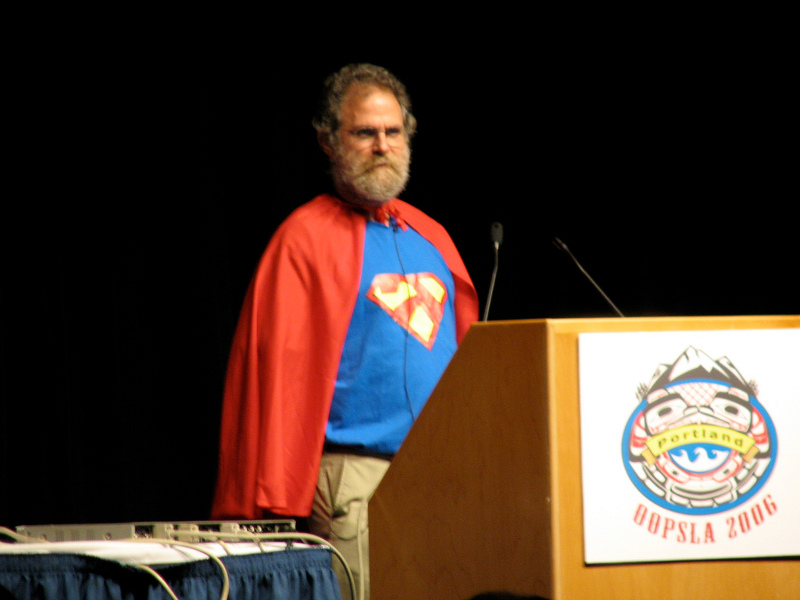
\includegraphics[height=8cm,width=12cm]{lambda-man.jpg}
\end{frame}

\begin{frame}
\frametitle{start with the types}
\pause
\begin{minipage}[t]{0.48\linewidth}
\begin{varblock}{value type}
\inputminted[mathescape,numbersep=5pt,fontsize=\footnotesize]{fsharp}{07-parservalue.fs}
\end{varblock}
\end{minipage}
\hfill%
\begin{minipage}[t]{0.52\linewidth}
\begin{varblock}{ parser return type}
\inputminted[mathescape,numbersep=5pt,fontsize=\footnotesize]{fsharp}{08-parsedvalue.fs}
\end{varblock}
\end{minipage}

\pause

\end{frame}
\begin{varblock}{ parser return type}
\inputminted[mathescape,numbersep=5pt,fontsize=\footnotesize]{fsharp}{06-parsectype.fs}
\end{varblock}

\begin{frame}
\resizebox{2cm}{!}{"9.12 "} 
\begin{itemize}
\item 9 is a number
\item but if we say so, what do we do for ".12" ?
\item the success of a parser depends on the rest of the string, not the first character
\end{itemize}
If it matters, it should be part of the returned type of a parser  !
\pause
\begin{varblock}{ parser return type}
\inputminted[mathescape,numbersep=5pt,fontsize=\footnotesize]{fsharp}{06-parsectypecomplete.fs}
\end{varblock}
\end{frame}

\begin{frame}

\inputminted[mathescape,numbersep=5pt,fontsize=\footnotesize]{fsharp}{06-parsectype.fs}
\begin{varblock}{ reading the parser type}

\begin{itemize} 
\item we start with  a list of token, the first n representing a $Val$ and the rest representing some other values
\item The parser's job is to give us back that $Val$ along with the "rest", assuming this VAL is emitted from the original input
\item the notion of "rest" is \textbf{dependent} on the $Val$ produced, this is why we include it in $ParseReturn$
\end{itemize}
\end{varblock}
\end{frame}

\begin{frame}
\frametitle{define simple block}
\end{frame}



\subsection{pickler combinator}




\begin{frame}
\frametitle{Paragraphs of Text}
Sed iaculis dapibus gravida. Morbi sed tortor erat, nec interdum arcu. Sed id lorem lectus. Quisque viverra augue id sem ornare non aliquam nibh tristique. Aenean in ligula nisl. Nulla sed tellus ipsum. Donec vestibulum ligula non lorem vulputate fermentum accumsan neque mollis.\\~\\

Sed diam enim, sagittis nec condimentum sit amet, ullamcorper sit amet libero. Aliquam vel dui orci, a porta odio. Nullam id suscipit ipsum. Aenean lobortis commodo sem, ut commodo leo gravida vitae. Pellentesque vehicula ante iaculis arcu pretium rutrum eget sit amet purus. Integer ornare nulla quis neque ultrices lobortis. Vestibulum ultrices tincidunt libero, quis commodo erat ullamcorper id.
\end{frame}

%------------------------------------------------

\begin{frame}
\frametitle{Bullet Points}
\begin{itemize}
\item Lorem ipsum dolor sit amet, consectetur adipiscing elit
\item Aliquam blandit faucibus nisi, sit amet dapibus enim tempus eu
\item Nulla commodo, erat quis gravida posuere, elit lacus lobortis est, quis porttitor odio mauris at libero
\item Nam cursus est eget velit posuere pellentesque
\item Vestibulum faucibus velit a augue condimentum quis convallis nulla gravida
\end{itemize}
\end{frame}

%------------------------------------------------

\begin{frame}
\frametitle{Blocks of Highlighted Text}
\begin{block}{Block 1}
Lorem ipsum dolor sit amet, consectetur adipiscing elit. Integer lectus nisl, ultricies in feugiat rutrum, porttitor sit amet augue. Aliquam ut tortor mauris. Sed volutpat ante purus, quis accumsan dolor.
\end{block}

\begin{block}{Block 2}
Pellentesque sed tellus purus. Class aptent taciti sociosqu ad litora torquent per conubia nostra, per inceptos himenaeos. Vestibulum quis magna at risus dictum tempor eu vitae velit.
\end{block}

\begin{block}{Block 3}
Suspendisse tincidunt sagittis gravida. Curabitur condimentum, enim sed venenatis rutrum, ipsum neque consectetur orci, sed blandit justo nisi ac lacus.
\end{block}
\end{frame}

%------------------------------------------------

\begin{frame}
\frametitle{Multiple Columns}
\begin{columns}[c] % The "c" option specifies centered vertical alignment while the "t" option is used for top vertical alignment

\column{.45\textwidth} % Left column and width
\textbf{Heading}
\begin{enumerate}
\item Statement
\item Explanation
\item Example
\end{enumerate}

\column{.5\textwidth} % Right column and width
Lorem ipsum dolor sit amet, consectetur adipiscing elit. Integer lectus nisl, ultricies in feugiat rutrum, porttitor sit amet augue. Aliquam ut tortor mauris. Sed volutpat ante purus, quis accumsan dolor.

\end{columns}
\end{frame}

%------------------------------------------------
\section{Second Section}
%------------------------------------------------

\begin{frame}
\frametitle{Table}
\begin{table}
\begin{tabular}{l l l}
\toprule
\textbf{Treatments} & \textbf{Response 1} & \textbf{Response 2}\\
\midrule
Treatment 1 & 0.0003262 & 0.562 \\
Treatment 2 & 0.0015681 & 0.910 \\
Treatment 3 & 0.0009271 & 0.296 \\
\bottomrule
\end{tabular}
\caption{Table caption}
\end{table}
\end{frame}

%------------------------------------------------

\begin{frame}
\frametitle{Theorem}
\begin{theorem}[Mass--energy equivalence]
$E = mc^2$
\end{theorem}
\end{frame}

%------------------------------------------------

\begin{frame}[fragile] % Need to use the fragile option when verbatim is used in the slide
\frametitle{Verbatim}
\begin{example}[Theorem Slide Code]
\begin{verbatim}

\frametitle{Theorem}
\begin{theorem}[Mass--energy equivalence]
$E = mc^2$
\end{theorem}

\end{verbatim}
\end{example}
\end{frame}

%------------------------------------------------

\begin{frame}
\frametitle{Figure}
Uncomment the code on this slide to include your own image from the same directory as the template .TeX file.
%\begin{figure}
%\includegraphics[width=0.8\linewidth]{test}
%\end{figure}
\end{frame}

%------------------------------------------------

\begin{frame}[fragile] % Need to use the fragile option when verbatim is used in the slide
\frametitle{Citation}
An example of the \verb|\cite| command to cite within the presentation:\\~

This statement requires citation \cite{p1}.
\end{frame}

%------------------------------------------------

\begin{frame}
\frametitle{References}
\footnotesize{
\begin{thebibliography}{99} % Beamer does not support BibTeX so references must be inserted manually as below
\bibitem[Smith, 2012]{p1} John Smith (2012)
\newblock Title of the publication
\newblock \emph{Journal Name} 12(3), 45 -- 678.
\end{thebibliography}
}
\end{frame}

%------------------------------------------------

\begin{frame}
\Huge{\centerline{The End}}
\end{frame}

%----------------------------------------------------------------------------------------

\end{document}
